\chapter{Chapter 1 Title}

\begin{chapterabstract}
    Use the chapterabstract environment, not the abstract environment, if you want to plant an abstract at the top of the chapter.
\end{chapterabstract}

\section{Introduction}

\begin{quote}
   Here's a quote environment, if needed.
\end{quote}
Here's a citation so we don't get a "no citation warning" \cite{GolV13}.
Here's a figure. 
\begin{figure}
    \begin{centering}
        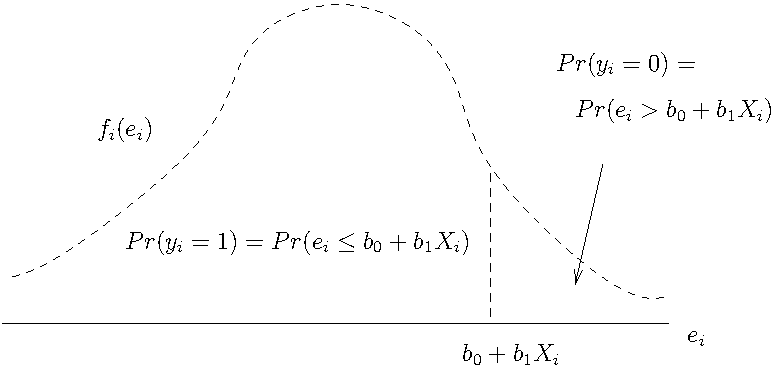
\includegraphics[scale=0.8]{chap_1/chap_1_figures/example_1.pdf}
    \par\end{centering}
    \caption{Figure for listoffigures  in the content page.}
    \label{fig:first_fig}
\end{figure}
Here how to reference a figure such as Figure \ref{fig:first_fig}.
\newpage
Here's a table.
\begin{table}
    \centering{}
    \begin{tabular}{|c|c|c|c|c|}
        \hline 
            & R: polr & R: lrm & SAS & Stata\tabularnewline
        \hline 
        \hline 
        $\hat{b}_{1}$ & -0.28 & -0.28 & 0.28 & -0.28\tabularnewline
        \hline 
        $\hat{\zeta}_{1}$ & -4.24 & 4.24 & -4.24 & -4.24\tabularnewline
        \hline 
        $\hat{\zeta}_{2}$ & -2.32 & 2.32 & -2.32 & -2.32\tabularnewline
        \hline 
    \end{tabular}
    \caption{Table for the listoftables in the contents page.}
    \label{tab:random_table}
\end{table}